\section{Results \& Discussion}
Figure~\ref{fig:dspcccref30} compared the reflectometry and SLD profiles from each of the different methods at an APM associated with a SP of \SI{30}{\milli\newton\per\meter}.\footnote{The data for the other APMs can be found in Appendix~\ref{refl2}, however, the trends are similar at all SPs.}
In addition, the $\chi^2$ between each of the models and the experimental data for each contrast at an APM associated with a SP of \SI{30}{\milli\newton\per\meter}, the average $\chi^2$ and standard deviation for each method are given in Table~\ref{tab:chi}.\footnote{The same data for other APMs is available Appendix~\ref{refl2}.}
%
\begin{figure}[t]
    \centering
    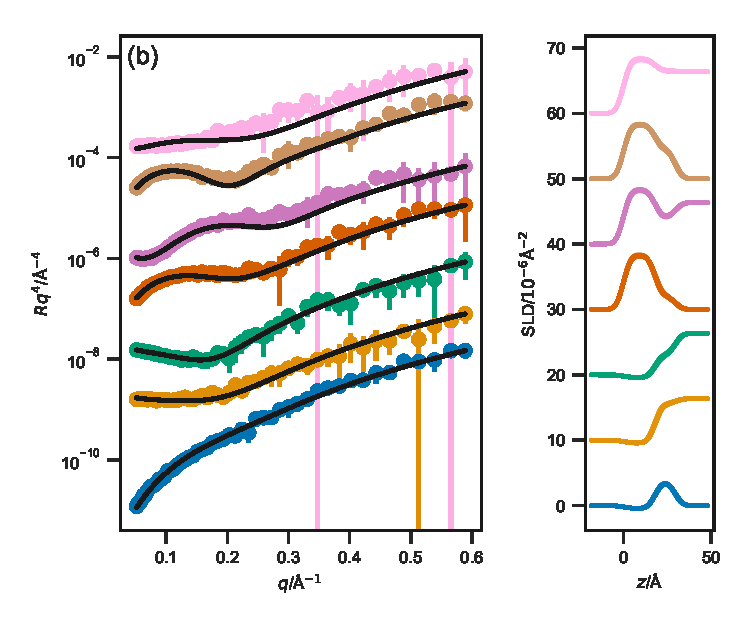
\includegraphics[width=0.49\textwidth]{reflectometry2/dspc_30_ref_sld}
    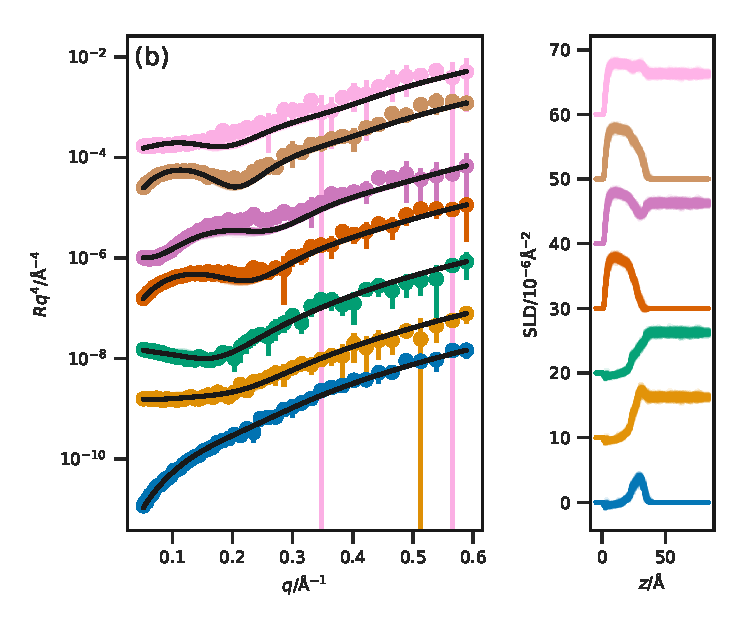
\includegraphics[width=0.49\textwidth]{reflectometry2/dspc_slipids_30_ref_sld}\\
    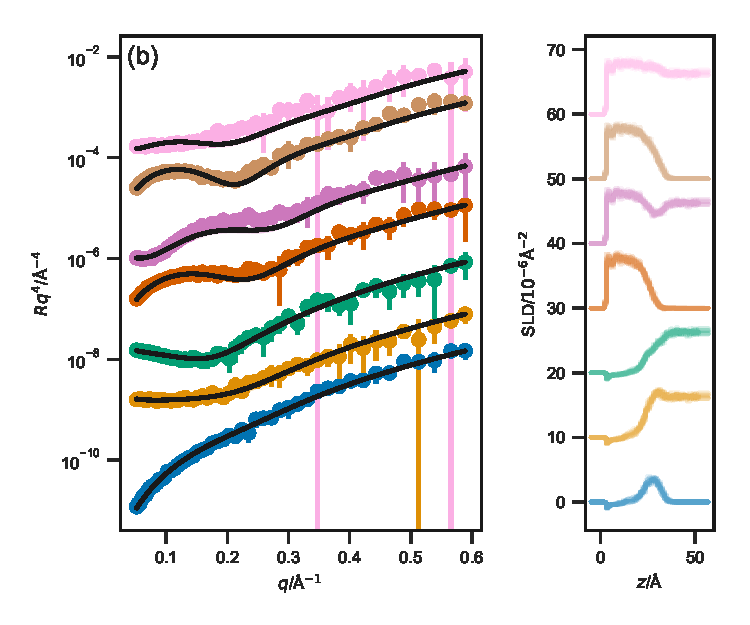
\includegraphics[width=0.49\textwidth]{reflectometry2/dspc_berger_30_ref_sld}
    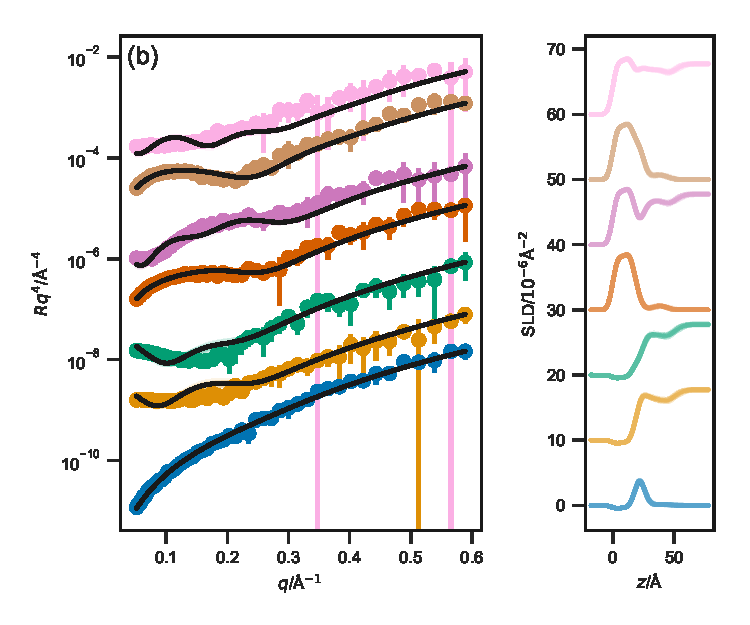
\includegraphics[width=0.49\textwidth]{reflectometry2/dspc_martini_30_ref_sld}
    \caption{The NR profiles (left) and SLD profiles (right) determined at an APM assocaited with a SP of \SI{30}{\milli\newton\per\meter} for; (a) the chemically-consistent model, (b) the Slipid all-atom potential model simulations, (c) the Berger united-atom potential model simulations, and (d) the MARTINI coarse-grained potential model simulations. From top-to-bottom the contrasts are as follows; d$_{83}$-\ce{D2O}, d$_{83}$-ACMW, d$_{70}$-\ce{D2O}, d$_{70}$-ACMW, h-\ce{D2O}, d$_{13}$-\ce{D2O}, d$_{13}$-ACMW. The different contrast NR profiles have been offset in the \emph{y}-axis by an order of magnitude and the SLD profiles offset in the \emph{y}-axis by \SI{10e-6}{\per\angstrom\squared}, for clarity.}
    \label{fig:dspcccref30}
\end{figure}
%
%
\begin{sidewaystable}
    \small
    \caption{The $\chi^2$ values for each of the reflectometry models at an APM associated with a SP of \SI{30}{\milli\newton\per\meter}.}
    \label{tab:chi}
    \begin{tabular}{l | l l l l}
        \toprule
        Contrast & Chemically-consistent & Slipids & Berger & MARTINI \\
        \midrule
        h-\ce{D2O} & \input{output/reflectometry2/dspc_30/dspc_30_hd2o_chi.txt} & \input{output/reflectometry2/dspc_30/dspc_slipids_30_hd2o_chi.txt} & \input{output/reflectometry2/dspc_30/dspc_berger_30_hd2o_chi.txt} & \input{output/reflectometry2/dspc_30/dspc_martini_30_hd2o_chi.txt} \\
        d$_{13}$-\ce{D2O} & \input{output/reflectometry2/dspc_30/dspc_30_d13d2o_chi.txt} & \input{output/reflectometry2/dspc_30/dspc_slipids_30_d13d2o_chi.txt} & \input{output/reflectometry2/dspc_30/dspc_berger_30_d13d2o_chi.txt} & \input{output/reflectometry2/dspc_30/dspc_martini_30_d13d2o_chi.txt} \\
        d$_{13}$-ACMW & \input{output/reflectometry2/dspc_30/dspc_30_d13acmw_chi.txt} & \input{output/reflectometry2/dspc_30/dspc_slipids_30_d13acmw_chi.txt} & \input{output/reflectometry2/dspc_30/dspc_berger_30_d13acmw_chi.txt} & \input{output/reflectometry2/dspc_30/dspc_martini_30_d13acmw_chi.txt} \\
        d$_{70}$-\ce{D2O} & \input{output/reflectometry2/dspc_30/dspc_30_d70d2o_chi.txt} & \input{output/reflectometry2/dspc_30/dspc_slipids_30_d70d2o_chi.txt} & \input{output/reflectometry2/dspc_30/dspc_berger_30_d70d2o_chi.txt} & \input{output/reflectometry2/dspc_30/dspc_martini_30_d70d2o_chi.txt} \\
        d$_{70}$-ACMW & \input{output/reflectometry2/dspc_30/dspc_30_d70acmw_chi.txt} & \input{output/reflectometry2/dspc_30/dspc_slipids_30_d70acmw_chi.txt} & \input{output/reflectometry2/dspc_30/dspc_berger_30_d70acmw_chi.txt} & \input{output/reflectometry2/dspc_30/dspc_martini_30_d70acmw_chi.txt} \\
        d$_{83}$-\ce{D2O} & \input{output/reflectometry2/dspc_30/dspc_30_d83d2o_chi.txt} & \input{output/reflectometry2/dspc_30/dspc_slipids_30_d83d2o_chi.txt} & \input{output/reflectometry2/dspc_30/dspc_berger_30_d83d2o_chi.txt} & \input{output/reflectometry2/dspc_30/dspc_martini_30_d83d2o_chi.txt} \\
        d$_{83}$-ACMW & \input{output/reflectometry2/dspc_30/dspc_30_d83acmw_chi.txt} & \input{output/reflectometry2/dspc_30/dspc_slipids_30_d83acmw_chi.txt} & \input{output/reflectometry2/dspc_30/dspc_berger_30_d83acmw_chi.txt} & \input{output/reflectometry2/dspc_30/dspc_martini_30_d83acmw_chi.txt} \\
        \midrule
        Average & \input{output/reflectometry2/dspc_30/dspc_30_all_chi.txt} & \input{output/reflectometry2/dspc_30/dspc_slipids_30_all_chi.txt} & \input{output/reflectometry2/dspc_30/dspc_berger_30_all_chi.txt} & \input{output/reflectometry2/dspc_30/dspc_martini_30_all_chi.txt} \\
        \bottomrule
    \end{tabular}
\end{sidewaystable}
%

\subsection{Traditional analysis}
The chemically-consistent model was used to determine the structure of the phospholipid monolayer, Table~\ref{tab:cc} gives the optimum values for the parameters that were varied in the model.
It is clear from this Table, that as the SP is increased, as expected, and as found previously,\autocite{mohwald_phospholipid_1990,vaknin_structural_1991} the overall thickness of the monolayer increases.
The thickness increase for the phospholipid tails may be associated with the straightening of the tails with respect to the interface normal, while the thickness increase of the head groups has been noted previously for DSPC.\autocite{hollinshead_effects_2009}
%
\begin{sidewaystable}
\small
  \caption{\ The values for the parameters allowed to vary in the fitting of the chemically-consistent model, at each SP measured.}
  \label{tab:cc}
  \begin{tabular}{llllll}
    \toprule
    SP/ & & & & & \\
    \si{\milli\newton\per\meter} & $d_h$/\si{\angstrom} & $d_t$/\si{\angstrom} & $\sigma_{t,h,s}$/\si{\angstrom} & $\phi_h$$\times10^{-2}$ & $V_t$/\si{\angstrom\cubed} \\
    \midrule
    20 & \input{output/reflectometry2/dspc_20/dspc_20-d_h_20.tex} & \input{output/reflectometry2/dspc_20/dspc_20-d_t_20.tex} & \input{output/reflectometry2/dspc_20/dspc_20_rough_20.tex} & \input{output/reflectometry2/dspc_20/dspc_20-phih_20.tex} & \input{output/reflectometry2/dspc_20/dspc_20-V_t_20.tex} \\
    30 & \input{output/reflectometry2/dspc_30/dspc_30-d_h_30.tex} & \input{output/reflectometry2/dspc_30/dspc_30-d_t_30.tex} & \input{output/reflectometry2/dspc_30/dspc_30_rough_30.tex} & \input{output/reflectometry2/dspc_30/dspc_30-phih_30.tex} & \input{output/reflectometry2/dspc_30/dspc_30-V_t_30.tex} \\
    40 & \input{output/reflectometry2/dspc_40/dspc_40-d_h_40.tex} & \input{output/reflectometry2/dspc_40/dspc_40-d_t_40.tex} & \input{output/reflectometry2/dspc_40/dspc_40_rough_40.tex} & \input{output/reflectometry2/dspc_40/dspc_40-phih_40.tex} & \input{output/reflectometry2/dspc_40/dspc_40-V_t_40.tex} \\
    50 & \input{output/reflectometry2/dspc_50/dspc_50-d_h_50.tex} & \input{output/reflectometry2/dspc_50/dspc_50-d_t_50.tex} & \input{output/reflectometry2/dspc_50/dspc_50_rough_50.tex} & \input{output/reflectometry2/dspc_50/dspc_50-phih_50.tex} & \input{output/reflectometry2/dspc_50/dspc_50-V_t_50.tex} \\
    \bottomrule
  \end{tabular}
\end{sidewaystable}
%

It would be anticipated that as the SP increases, there would be a corresponding decrease in the volume fraction of solvent in the head group.\autocite{bayerl_specular_1990}
However, for DSPC, the volume fraction of the solvent appears to be constant (or even increase slightly) with increasing SP.
This is due to the decision to constrain the volume of the phospholipid head, which may decrease with increasing SP.

Hollinshead \emph{et al.}\autocite{hollinshead_effects_2009} suggest a tail volume of \SI{972}{\angstrom\cubed} from the density data.
However, the values found in this work are substantially lower, at \SI{\sim850}{\angstrom\cubed}.
This reduction, of \SI{\sim12}{\percent}, agrees well with the work of Campbell \emph{et al.}\autocite{campbell_structure_2018} and Small,\autocite{small_lateral_1984} which suggest that under the SP investigated in this work a reduction of the tail volume of up to \SI{15}{\percent} may be observed.
The model layer structure from the chemically-consistent method provides a satisfactory description of the monolayer structure.
However, the use of an MD-driven analysis method may provide greater insight into the chemical nature of the monolayer.

\subsection{MARTINI}
\label{sec:martanal}
Initially, the MARTINI coarse-grained simulations were analysed with a layer thickness of \SI{1}{\angstrom} and an interfacial roughness of \SI{0}{\angstrom}, in a similar fashion to the other potential models.
However, as can be seen in Figure~\ref{fig:martorder} there is a clear ordering effect present in the MARTINI water, despite the use of the polarised water model.
The effect of this ordering on the SLD profile, and therefore the reflectometry profile, can be reduced by using a larger layer thickness and introducing an interfacial roughness.
Therefore, in the results discussed below the MARTINI potential model simulation were analysed using a layer thickness of \SI{4}{\angstrom} and an interfacial roughness of \SI{0.4}{\angstrom}.
It is noted that this structuring may be reduced through the use of a less ordered wall\autocite{koutsioubas_combined_2016} at the extreme of the simulation cell, however, the aim was to reproduce the experimental conditions using off-the-shelf tools and this would require custom modifications not easily available.
Alternatively, it may be possible to effect the presence of this structuring through the inclusion of \SI{\sim 10}{\percent} of antifreeze MARTINI beads alongside the normal MARTINI water.
However, this method has been noted to also give structuring effects in the presence on an ordered wall.\autocite{marrink_comment_2010}
%
\begin{figure}[t]
    \centering
    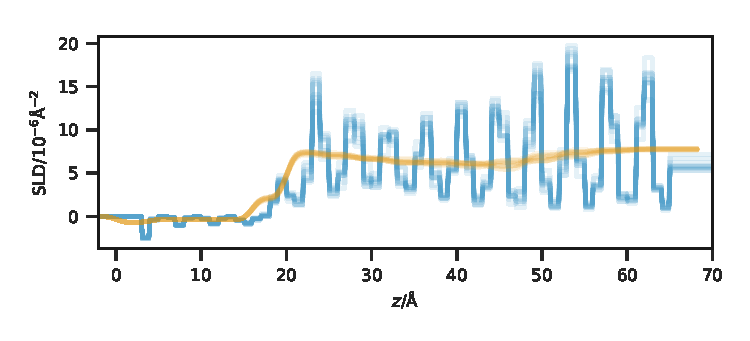
\includegraphics[width=\textwidth]{reflectometry2/martini_order}
    \caption{A comparison of the scattering length density profile for the MARTINI potential model simulations at an APM associated with a SP of \SI{30}{\milli\newton\per\meter}; the blue line shows the data where the layer thickness was \SI{1}{\angstrom} and no interfacial roughness and the orange line shows that with a layer thickness of \SI{4}{\angstrom} and a roughness of \SI{0.4}{\angstrom}.}
    \label{fig:martorder}
\end{figure}
%

It can be seen from Table~\ref{tab:chi} and Figure~\ref{fig:dspcccref30} that even with the larger layer thickness and adding interlayer roughness, the MARTINI potential model simulations do not effectively reproduce the reflectometry profile.
Furthermore, it is noted that the agreement with the contrasts containing \ce{D2O} is particularly poor.
This is most likely an artefact of the structuring effect mentioned above which cannot be completely removed.

However, the agreement for the samples where the contrast uses ACMW, where the water is effectively removed from the SLD profile is also poor.
This indicates that there are other artefacts limiting the applicability of the MARTINI potential model.
One such artefact is clear from investigating the calculated length of the hydrocarbon tail from the MARTINI simulation, at an APM associated with an SP of \SI{30}{\milli\newton\per\meter}, which was found to be \input{output/reflectometry2/dspc_30/dspc_martini_30_dt.txt}~\si{\angstrom}, significantly less than the \SI{24.3}{\angstrom} estimated by the Tanford equation.\autocite[which has the form $t_t = (1.5 + 1.265)n_c$ \AA, where $t_t$ is the length and $n_c$ is the number of carbon atoms]{tanford_hydrophobic_1980}
This is due to the nature of the MARTINI's 4-to-1 beading process, as DSPC has a hydrocarbon tail consisting of 18 carbon atoms, and it is not possible to bead such a chain accurately with the MARTINI potential model.
In this work, a MARTINI phospholipid molecule was used with 4 MARTINI beads making up the chain.\footnote{This corresponds to an all-atom hydrocarbon chain of 16 atoms.}
Applying the Tanford equation to a hydrocarbon chain of such a length results in an anticipated length of \SI{18.7}{\angstrom}, which agrees better with that found from the simulation.

In addition to the disagreement from the tail beading process, there is also a clear problem with respect to the solvation of the head layer by polarisable water beads.
It can be seen that the number of water molecules per head group in the MARTINI potential model is typically \input{output/reflectometry2/dspc_30/dspc_martini_30_wph.txt}, this is the value at an APM associated with an SP of \SI{30}{\milli\newton\per\meter}.
The chemically-consistent model, however, gives a value of \input{output/reflectometry2/dspc_30/dspc_30-wph_30.tex}.
It is clear that the 4-to-1 beading present in the MARTINI potential model is creating water molecules that are too large to intercalate into the head layer structure, causing a reduction in the number of waters per head group.

The requirement for a 4-to-1 beading strategy for the MARTINI potential model is a significant weakness.
A better method may be limiting experiments to a system that can be modelled exactly or the use of a different beading model.
However, I am not aware of an off-the-shelf coarse-grained potential model that would easily offer the exact beading of DSPC.

\subsection{Comparison with other simulations}
Table~\ref{tab:chi} shows that both the Slipid and Berger potential model simulations agree well with the experimental data, with the Slipid potential model offering a slight improvement over the Berger.
The quality of agreement between these higher-resolution potential models and the chemically-consistent model is relatively similar.
However, the chemically-consistent model still offers a better fit to the experimental data than those determined from MD simulation.

The result that the chemically-consistent model offers better agreement with the data than those from even all-atom simulations is to be expected by considering the level of constraint present implicitly when determining the reflectometry profile directly from the simulation.
While the chemically-consistent model constrains the layer model to ensure that the number of phospholipid head groups is the same as the pairs of tail groups, those from MD simulation have more realistic chemical constraints present from the potential model.\footnote{Such as the bonding between atoms, and the non-bonded potentials.}
The quality of the agreement from this multi-modal approach is sufficient for such a method to be applied regularly to the analysis of NR.

Both the Slipid and Berger potential model simulations produced values for the tail length that were in better agreement with that from the Tanford equation than the MARTINI potential model simulations.
For the Slipid potential model, with simulations at an APM associated with an SP of \SI{30}{\milli\newton\per\meter} the tail length was found to be \input{output/reflectometry2/dspc_30/dspc_slipids_30_dt.txt}~\si{\angstrom}, while for the Berger potential model, at the same APM, a value of \input{output/reflectometry2/dspc_30/dspc_berger_30_dt.txt}~\si{\angstrom} was obtained.
Neither is quite as large as the \SI{24.3}{\angstrom} from the Tanford equation.\footnote{It should be noted that this value is considered a theoretical maximum for a fully extended carbon chain, which is unlikely to occur, in a liquid phase monolayer, in reality, due to entropic considerations.}

Using the MD simulations and the chemically-consistent model, it is possible to compare the number of water molecules per head group.
From the Slipid and Berger potential model simulations, the number of water molecules per head group at an APM associated with an SP of \SI{30}{\milli\newton\per\meter} was found to be \input{output/reflectometry2/dspc_30/dspc_slipids_30_wph.txt} and \input{output/reflectometry2/dspc_30/dspc_berger_30_wph.txt} respectively.
These are in good agreement with the value of \input{output/reflectometry2/dspc_30/dspc_30-wph_30.tex} found from the chemically-consistent model, using Equation~\ref{equ:wph}.

It should be noted that to obtain the \SI{50}{\nano\second} production run simulation using the all-atom Slipid potential model required over 13 days of using 32 cores of the SCARF computing resource.
This is non-trivial and therefore not necessarily applicable to all NR measurements.
However, the use of a \SI{2}{\femto\second} timestep could reduce this time significantly.
Additionally, Figure \ref{fig:short} shows the results from the first \SI{5}{\nano\second} of the Slipid potential model simulations, at an APM associated with an SP of \SI{30}{\milli\newton\per\meter}, and already good agreement with the data is apparent.
It is important to acknowledge that the length of simulation required may be extremely system specific.
Furthermore, recent developments of MD simulations of graphical processing units\footnote{Abbreviated to GPUs.} may allow for significant speed up of the simulations.
The nearly as accurate Berger potential model simulations, only approximately 2 days of the same compute resource was required.
This suggests that by using a larger timestep, shorter simulations, and the power of GPU-based MD engines, it may be possible to run these simulations alongside experiments at large facilities to aid interpretation and analysis.
%
\begin{figure}[t]
    \forcerectofloat
    \centering
    \includegraphics[width=0.85\textwidth]{reflectometry2/dspc_slipids_30_ref_sld_short}
    \caption{The reflectometry and SLD profiles obtained from the first \SI{5}{\nano\second} of the Slipid potential model simulation, at an APM associated with a SP of \SI{30}{\milli\newton\per\meter}. From top-to-bottom the contrasts are as follows; \ce{d_{83}}-\ce{D2O}, \ce{d_{83}}-ACMW, \ce{d_{70}}-\ce{D2O}, \ce{d_{70}}-ACMW, h-\ce{D2O}, \ce{d_{13}}-\ce{D2O}, \ce{d_{13}}-ACMW. The different contrast reflectometry profiles have been offset in the \emph{y}-axis by an order of magnitude and the SLD profiles offset in the \emph{y}-axis by \SI{10e-6}{\per\square\angstrom}, for clarity.}
    \label{fig:short}
\end{figure}
%

\subsection{Using the Slipid potential model simulations to improve the monolayer model}
Despite the chemically-consistent model offering a small improvement in agreement over the Slipid potential model simulation, it is possible to use the MD simulations to improve this model.
A possible improvement can be found from considering Figure~\ref{fig:waters30}, which shows the solvent penetration of the phospholipid heads, using the intrinsic surface approach to remove the effect of the interfacial roughness.
It is clear that the plot is not step-wise as is obtained from the uniform solvation model that is commonly used in traditional layer models.
Nor is the distribution sigmoidal, as there is a small deviation in the region of the ester group of the phospholipid heads.
This is either due to the hydrophilic interaction of the carbonyl moiety or from pockets of water forming at the air-water interface.
Regardless of the mechanism, this suggests that a different solvation model should be considered for a realistic description of the solvent penetration.
%
\begin{figure}[t]
  \forceversofloat
    \centering
    \includegraphics[width=\textwidth]{reflectometry2/water_30}
    \caption{The simulation time-averaged intrinsic density profile of the water molecules (blue dots), and phospholipid components (head groups: green dots, tail groups: red dots) at an APM associated with a SP of \SI{30}{\milli\newton\per\meter}, where the phosphorus atoms of the phospholipid heads create the intrinsic surface at $z=0$\si{\angstrom}, and the equivalent number density from the chemically-consistent model (orange line).}
    \label{fig:waters30}
\end{figure}
%

%
\begin{table}[b]
\forceversofloat
\centering
\small
  \caption{\ The mean, \SI{95}{\percent} quantile, and their spread for the \emph{z}-dimension position of atoms representative of difference parts of the phospholipid, at an APM associated with a SP of \SI{30}{\milli\newton\per\meter}.}
  \label{tab:spread2}
  \begin{tabular}{llll}
    \toprule
    Position & Mean/\si{\angstrom} & \SI{95}{\percent} quantile/\si{\angstrom} & Spread/\si{\angstrom} \\
    \midrule
    Start-Head & \input{output/reflectometry2/dspc_30/slipids_mean_N_30.txt} & \input{output/reflectometry2/dspc_30/slipids_uq_N_30.txt} & \input{output/reflectometry2/dspc_30/slipids_position_N_30.txt} \\
    Mid-Head & \input{output/reflectometry2/dspc_30/slipids_mean_P_30.txt} & \input{output/reflectometry2/dspc_30/slipids_uq_P_30.txt} & \input{output/reflectometry2/dspc_30/slipids_position_P_30.txt} \\
    End-Head & \input{output/reflectometry2/dspc_30/slipids_mean_C2_30.txt} & \input{output/reflectometry2/dspc_30/slipids_uq_C2_30.txt} & \input{output/reflectometry2/dspc_30/slipids_position_C2_30.txt} \\
    \midrule
    Start-Tail 1 & \input{output/reflectometry2/dspc_30/slipids_mean_C21_30.txt} & \input{output/reflectometry2/dspc_30/slipids_uq_C21_30.txt} & \input{output/reflectometry2/dspc_30/slipids_position_C21_30.txt} \\
    Start-Tail 2 & \input{output/reflectometry2/dspc_30/slipids_mean_C31_30.txt} & \input{output/reflectometry2/dspc_30/slipids_uq_C31_30.txt} & \input{output/reflectometry2/dspc_30/slipids_position_C31_30.txt} \\
    Mid-Tail 1 & \input{output/reflectometry2/dspc_30/slipids_mean_C29_30.txt} & \input{output/reflectometry2/dspc_30/slipids_uq_C29_30.txt} & \input{output/reflectometry2/dspc_30/slipids_position_C29_30.txt} \\
    Mid-Tail 2 & \input{output/reflectometry2/dspc_30/slipids_mean_C39_30.txt} & \input{output/reflectometry2/dspc_30/slipids_uq_C39_30.txt} & \input{output/reflectometry2/dspc_30/slipids_position_C39_30.txt} \\
    End-Tail 1 & \input{output/reflectometry2/dspc_30/slipids_mean_8C21_30.txt} & \input{output/reflectometry2/dspc_30/slipids_uq_8C21_30.txt} & \input{output/reflectometry2/dspc_30/slipids_position_8C21_30.txt} \\
    End-Tail 2 & \input{output/reflectometry2/dspc_30/slipids_mean_8C31_30.txt} & \input{output/reflectometry2/dspc_30/slipids_uq_8C31_30.txt} & \input{output/reflectometry2/dspc_30/slipids_position_8C31_30.txt} \\
    \bottomrule
  \end{tabular}
\end{table}
%
Figure~\ref{fig:waters30} also shows that without the presence of the roughness, the distribution of the head groups is relatively normal.
This agrees well with the model used previously to fit the experimental data by Hollinshead \emph{et al.},\autocite{hollinshead_effects_2009} where Gaussian functions were used to describe the phospholipid head and tail groups.
However, the tail group distribution is not Gaussian and this previous method failed to include any additional factors to account for interfacial roughness.
Previous work has suggested that when only a single phospholipid type is present, the roughness between the layers should be conformal in nature, that is it should be carried uniformly through the layers.\autocite{kozhevnikov_general_2012,campbell_structure_2018}
However, from the investigation of the SLD profiles in Figure~\ref{fig:dspcccref30}(b), it appears that the roughness between the phospholipid tails and the air is dramatically different from that at the phospholipid head-water interface.
In an effort to quantify the interfacial roughness in the simulations, the method outlined in Section~\ref{sec:traj} was used.
The values for the mean, \SI{95}{\percent} quantile, and the spread between these for the \emph{z}-dimension position for atoms representative of the start, middle, and end of each of the phospholipid head and tails are given in Table~\ref{tab:spread2}, for each the APM associated with a SP of \SI{30}{\milli\newton\per\meter}.\footnote{Similar data at other SPs can be found in Appendix~\ref{refl2}.}
From this table, it is clear that at the very start of the phospholipid molecule\footnote{At the head group.} the roughness is very large with a value of \SI{\sim10}{\angstrom} for the nitrogen atom.
However, this decreases slightly within the phospholipid head, reaching a value of \input{output/reflectometry2/dspc_30/slipids_position_C2_30.txt}\si{\angstrom} for the end of the head group.
There is then a substantial decrease noted in the phospholipid tail, going from \SI{\sim8.5}{\angstrom} at the start of the tail to \SI{\sim1.5}{\angstrom} at the end.
This indicates the presence of a highly non-conformal roughness in the phospholipid monolayer of a single phospholipid type and therefore in future, it is important to consider this possibility in the use of model layer structure method.
